% Solutions to the exercises of Chapter 23. Numbers: code/solutions/sol23.py
\documentclass[../solutions_manual.tex]{subfiles}
\begin{document}
\ifSubfilesClassLoaded{\setcounter{chapter}{22}}{}% NN-1 when built standalone
\setcounter{chapter}{22}% NN-1, so this chapter is numbered NN
\chapter{Tracking Structural Change Over Time}\label{sol23}

Every number below is printed by \texttt{python3 code/solutions/sol23.py}. The sources, all in \path{data/processed} and retrieved 2026-11-05, are:
\begin{itemize}
\item INE's input--output matrices (base 1990) and supply--use tables (base 2017), as domestic flow matrices on the book's 12 sectors (\path{bolivia_Z/}, \path{bolivia_io_summary.csv}, \path{bolivia_io_pi.csv});
\item the OECD ICIO domestic blocks, 2021 and 2023 editions, on ISIC-based 12 sectors (\path{oecd_io_summary.csv});
\item Growth Lab ECI, HS92 (\path{eci_facts.csv}).
\end{itemize}
Unless stated otherwise, $\Gamma$ is that of $W^P = D^{-1}A$ with domestic flows and the diagonal kept. EH microdata were not fetched, so no $\sigma_B$ is reported.

%% ---------------------------------------------------------------------
\exercisesolution{23.1}{Bolivia's trajectory}

\solpart{Method}
\begin{enumerate}
\item For each year, take INE's domestic industry $\times$ industry flow matrix $Z_t$ at basic prices (12 book sectors).
\item Drop sectors without intermediate purchases or sales: domestic services always, and public administration in years without a published make matrix.
\item Form $W^P_t$ and compute $\Gamma_t$, $\bpi_t$ and $G(\bpi_t)$.
\item Keep base 1990 (2000--2014) and base 2017 (2017--2019) as separate series.
\item Repeat with sales shares ($D^{-1}Z$) and with the diagonal set to zero before normalizing.
\end{enumerate}
$\sigma_{B,t}$ would be computed from each year's EH as in Exercise~19.1; the microdata were not fetched.

\solpart{The trajectory (input shares, diagonal kept)}
\begin{center}\small
\begin{tabular}{lcccccccccc}
\toprule
& 2000 & 2002 & 2003 & 2004 & 2005 & 2006 & 2007 & 2009 & 2013 & 2014 \\
\midrule
$\Gamma_t$ & 0.494 & 0.501 & 0.514 & 0.524 & 0.502 & 0.518 & 0.489 & 0.504 & 0.484 & 0.361 \\
$G(\bpi_t)$ & 0.420 & 0.447 & 0.444 & 0.385 & 0.366 & 0.424 & 0.350 & 0.353 & 0.371 & 0.352 \\
\bottomrule
\end{tabular}
\end{center}
The other base-1990 years are 2001 ($0.493$, $0.410$), 2008 ($0.486$, $0.341$), 2011 ($0.478$, $0.369$) and 2012 ($0.506$, $0.379$). On base 2017: 2017 ($0.506$, $0.446$), 2018 ($0.493$, $0.444$), 2019 ($0.467$, $0.445$).
\begin{center}
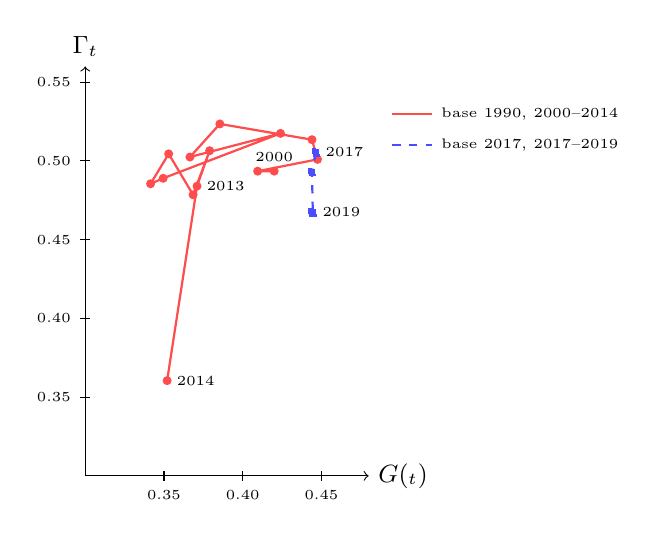
\begin{tikzpicture}[scale=1]
%% x = 20 (G(pi) - 0.30), y = 20 (Gamma - 0.30); coordinates printed by code/solutions/sol23.py
\draw[->] (0,0) -- (3.6,0) node[right, font=\small] {$G(\bpi_t)$};
\draw[->] (0,0) -- (0,5.2) node[above, font=\small] {$\Gamma_t$};
\foreach \x/\l in {1/0.35, 2/0.40, 3/0.45} {\draw (\x,-0.06) -- (\x,0.06); \node[below, font=\tiny] at (\x,-0.06) {\l};}
\foreach \y/\l in {1/0.35, 2/0.40, 3/0.45, 4/0.50, 5/0.55} {\draw (-0.06,\y) -- (0.06,\y); \node[left, font=\tiny] at (-0.06,\y) {\l};}
\draw[red!70, thick, mark=*, mark size=1.2pt] plot coordinates {(2.40,3.87) (2.19,3.87) (2.95,4.02) (2.88,4.27) (1.71,4.47) (1.33,4.05) (2.48,4.35) (0.99,3.78) (0.83,3.71) (1.06,4.09) (1.37,3.57) (1.58,4.13) (1.42,3.68) (1.04,1.21)};
\draw[blue!70, thick, dashed, mark=square*, mark size=1.2pt] plot coordinates {(2.93,4.11) (2.88,3.86) (2.89,3.35)};
\node[font=\tiny, above] at (2.40,3.87) {2000};
\node[font=\tiny, right] at (1.42,3.68) {2013};
\node[font=\tiny, right] at (1.04,1.21) {2014};
\node[font=\tiny, right] at (2.93,4.11) {2017};
\node[font=\tiny, right] at (2.89,3.35) {2019};
\draw[red!70, thick] (3.9,4.6) -- (4.4,4.6); \node[right, font=\tiny] at (4.4,4.6) {base 1990, 2000--2014};
\draw[blue!70, thick, dashed] (3.9,4.2) -- (4.4,4.2); \node[right, font=\tiny] at (4.4,4.2) {base 2017, 2017--2019};
\end{tikzpicture}
\end{center}

\solpart{Which coordinates move?} On base 1990, 2000--2013, $\Gamma$ barely moves ($-0.010$) while $G(\bpi)$ falls by $0.049$. The year-to-year co-movement of the two is weak and positive (correlation $+0.401$ over 2000--2014). Including the outlier year 2014 changes the picture: $\Gamma$ then falls by $0.133$. On base 2017, $\Gamma$ falls ($-0.038$, 2017--2019) and $G(\bpi)$ is flat ($-0.002$).

\solpart{Robustness to normalization} Changes over the same periods:
\begin{center}\small
\begin{tabular}{lcccc}
\toprule
& \multicolumn{2}{c}{2000--2013 (base 1990)} & \multicolumn{2}{c}{2017--2019 (base 2017)} \\
& $\Delta\Gamma$ & $\Delta G(\bpi)$ & $\Delta\Gamma$ & $\Delta G(\bpi)$ \\
\midrule
input shares & $-0.010$ & $-0.049$ & $-0.038$ & $-0.002$ \\
input shares, zero diagonal & $+0.044$ & $+0.025$ & $-0.018$ & $-0.003$ \\
sales shares & $-0.204$ & $+0.039$ & $+0.005$ & $+0.001$ \\
sales shares, zero diagonal & $+0.000$ & $-0.032$ & $-0.007$ & $+0.000$ \\
\bottomrule
\end{tabular}
\end{center}
\emph{The direction of change does not survive.} Over 2000--2013 the sign of $\Delta\Gamma$ is negative for two variants and non-negative for the other two, and $\Delta G(\bpi)$ has both signs as well. Over 2017--2019 three of the four variants agree on a falling $\Gamma$ (sales shares give $+0.005$). The magnitudes are of the order of the year-to-year noise (Exercise~23.2), except the sales-share fall of $0.204$, which is driven by the composition of sales. The trajectory is not a robust object at this aggregation: report a band across variants, not a single line.

%% ---------------------------------------------------------------------
\exercisesolution{23.2}{Structural break detection}

\solpart{Criterion} Definition~\ref{ch23:def:break} with $\hat\sigma_{\Delta\Gamma}$ estimated from the 9 quiet changes of 1989--1997: $\hat\sigma = 0.0090$, so $2\hat\sigma = 0.0181$. On base 1990 the year-to-year changes include $+0.101$ (1999), $-0.148$ (2000), $-0.021$ (2005), $-0.029$ (2007), $+0.019$ (2009), $+0.028$ (2012), $-0.022$ (2013) and $-0.123$ (2014). There is no 2010 table, so 2011 has no change. At $k = 2$ the flagged years are:
\begin{itemize}
\item base 1990: 1999, 2000, 2005, 2007, 2009, 2012, 2013 and 2014;
\item base 2017, with the same $\hat\sigma$: 2019 ($-0.026$), 2020 ($-0.049$), 2022 ($-0.032$), 2023 ($-0.019$) and 2024 ($+0.038$).
\end{itemize}
At $k = 2$ the criterion flags a third of all years. A threshold calibrated on a quiet decade is too tight for a series whose construction changes.

\solpart{Bootstrap band} The noise model is an assumption, standing in for INE's unpublished revision ranges: every cell of $Z_t$ is multiplied by independent lognormal noise with mean one and coefficient of variation 10\%, and $\Gamma_t$ is recomputed ($B = 300$ per year). The mean bootstrap s.d.\ of $\Gamma_t$ is $0.0220$. The 95\% bootstrap band of $\Delta\Gamma_t$ excludes zero only for 1999 ($[+0.030, +0.211]$), 2000 ($[-0.253, -0.070]$) and 2014 ($[-0.188, -0.076]$). Every other flagged year, including all of base 2017 (for example 2020, $[-0.104, +0.009]$), is within noise. \emph{Breaks surviving both criteria: 1999, 2000 and 2014.} None corresponds to a policy event. 1999 and 2000 lie in a run of diagonal-make years, and 2014 is the last year of the base. These are the construction effects the chapter identifies (Example~\ref{ch23:ex:epochs}). Note that cell noise does not capture construction error, such as a missing make matrix. The bootstrap tests measurement noise, not methodology.

\solpart{$\tau_1$ and $\Gamma^{(5)}$} Products require a common node set, so we use the 10 sectors defined in every base-1990 year (dropping domestic services and public administration).
\begin{itemize}
\item \emph{Dobrushin coefficient.} $\tau_1(W_t)$ ranges over $0.722$--$0.847$. Every $W_t$ is scrambling, $1 - \tau_1 \ge 0.153$, so Hajnal's condition holds trivially (Proposition~\ref{ch23:prop:hajnal}). The bound $\Gamma_t \ge 1 - \tau_1(W_t)$ of Proposition~\ref{ch23:prop:dobrushin} holds in every year, but it is loose ($0.15$--$0.28$ against $\Gamma_t \approx 0.5$). $\tau_1$ moves little and shows no break.
\item \emph{Realized-product gap.} $\Gamma^{(5)}_t = 1 - |\lambda_2(W_{t+4}\cdots W_t)|^{1/5}$, over windows of five consecutive years, ranges over $0.506$--$0.578$. It declines smoothly: $0.572$ for the 1990 window, $0.558$ for 1996 (which contains 1999--2000), $0.508$ for 2001 and $0.506$ for 2005. The per-period spike $\Gamma_{1999} = 0.642$ is averaged away. Windows containing 1999 average $0.547$, the others $0.542$.
\end{itemize}
\emph{Do they tell the same story?} No. $\Gamma_t$ shows spikes. The realized product, which is what a dynamic process driven by the sequence $W_t$ actually experiences, shows a gradual decline of about $0.07$ over 15 years with no break. This is the warning of Remark~\ref{ch23:rem:product_counterexample} in reverse: here the per-period gap \emph{exaggerates} the instability.

%% ---------------------------------------------------------------------
\exercisesolution{23.3}{Structural velocity}

\solpart{Results} Velocities per decade ($v_\Gamma$ by endpoints and by OLS on all years in the window), with $\Delta$ECI over the same years:
\begin{center}\small
\begin{tabular}{llccccc}
\toprule
& window & $\Gamma_{t_0} \to \Gamma_T$ & endpoint & OLS & $\Delta$ECI \\
\midrule
Chile & 1995--2014 (ICIO 2021) & $0.467 \to 0.640$ & $+0.091$ & $+0.079$ & $-0.088$ \\
Chile & 2011--2020 (ICIO 2023) & $0.449 \to 0.544$ & $+0.107$ & $+0.090$ & $-0.190$ \\
Peru & 1995--2014 (ICIO 2021) & $0.621 \to 0.507$ & $-0.060$ & $-0.100$ & $-0.065$ \\
Peru & 2011--2020 (ICIO 2023) & $0.448 \to 0.405$ & $-0.047$ & $-0.053$ & $-0.205$ \\
Bolivia & 1995--2014 (base 1990) & $0.578 \to 0.361$ & $-0.115$ & $-0.067$ & $-0.490$ \\
Bolivia & 1995--2013 (excl.\ 2014) & $0.578 \to 0.484$ & $-0.052$ & $-0.050$ & $-0.433$ \\
Bolivia & 2017--2024 (base 2017) & $0.506 \to 0.419$ & $-0.124$ & $-0.161$ & $+0.270$ \\
\bottomrule
\end{tabular}
\end{center}
The endpoint values reproduce \path{gamma_velocity.csv} (checked).

\solpart{Sign stability} Chile's velocity is positive in both windows and Peru's negative in both, by both estimators. No single base spans 2011--2020 for Bolivia. The partial windows give $-0.392$ (2011--2014, 4 points) and $-0.292$ (2017--2020, 4 points, including the pandemic). Four-point slopes are noise. Bolivia's two bases agree on the sign, but the 1995--2014 endpoint value is inflated by the 2014 outlier ($-0.115$ against $-0.052$ without it).

\solpart{Comparison with ECI and interpretation} The sign of $v_\Gamma$ is unrelated to the change in complexity. Chile has the fastest-rising $\Gamma$ in the sample and a falling ECI in both windows. Peru has a falling $\Gamma$ and a falling ECI. Bolivia's ECI rose ($+0.270$) over 2017--2024 while its $\Gamma$ fell fastest. That two countries kept their sign here does not rescue $v_\Gamma$: Korea and Argentina flip (Example~\ref{ch23:ex:velocities}). $v_\Gamma$ measures the change in the mixing speed of an aggregated input-share matrix. It is not a measure of development, which concerns capabilities (complexity, productivity, distribution). A positive $v_\Gamma$ can come from changes unrelated to capabilities, for example a concentration of input flows on a commodity hub.

%% ---------------------------------------------------------------------
\exercisesolution{23.4}{Structural-cyclical decomposition}

\solpart{Data and method} The series is $\pi_{\text{gas},t}$ on base 1990, book12, domestic, input shares, 1988--2014. It rises from $0.025$ (1988) to $0.047$ (2003), $0.074$ (2005), $0.087$ (2007), $0.085$ (2013) and $0.117$ (2014). There is no 2010 table. We use an HP filter with a missing observation: the trend $\tau_t$ is defined on every year 1988--2014, and the fit term uses observed years only,
\[
\min_{\tau}\sum_{t\ \text{observed}}(\pi_t - \tau_t)^2 + \lambda\sum_{t}(\tau_{t+1} - 2\tau_t + \tau_{t-1})^2 .
\]
This equals the ordinary HP filter when nothing is missing (checked on 1988--2009). It interpolates 2010, giving $\tau_{2010} = 0.0841$ at $\lambda = 100$.

\solpart{Results} The observed rise from 2003 to 2013 is $+0.0380$ ($0.0467 \to 0.0847$). The structural share is $(\tau_{2013} - \tau_{2003})/(\pi_{2013} - \pi_{2003})$:
\begin{center}\small
\begin{tabular}{lccc}
\toprule
& $\lambda = 6.25$ & $\lambda = 100$ & $\lambda = 400$ \\
\midrule
with 2014 & 1.179 & 1.217 & 1.180 \\
without 2014 & 0.880 & 1.007 & 1.029 \\
\bottomrule
\end{tabular}
\end{center}
At $\lambda = 100$ with 2014, the trend runs from $0.0507$ (2003) to $0.0969$ (2013). The gain-$\tfrac12$ cutoff periods are $9.8$, $19.8$ and $28.0$ years.

\solpart{Interpretation} Taken at face value, the filter calls essentially \emph{all} of the rise structural ($88\%$ to $122\%$). That is an artefact of the window. A rise that lasts a decade and does not reverse \emph{within the sample} has most of its power below the cutoff frequency, so any HP trend absorbs it. Shares above one appear because the 2014 spike pulls the trend's endpoint above the observed 2013 value. Dropping 2014 lowers the share at $\lambda = 6.25$ from $1.179$ to $0.880$. The persistence criterion of Definition~\ref{ch23:def:decomposition} can classify the boom only with post-boom data on the same base. These do not exist: the base-1990 series ends in 2014.

The composition of the node set is not the problem. $N$ alternates between 10 and 11 as public administration enters and leaves, but on the common 10-sector set $\pi_{\text{gas}}$ is almost identical ($0.047$ in 2003, $0.086$ in 2013, $0.119$ in 2014), and the share at $\lambda = 100$ is $1.216$.

\solpart{Why the base-2017 years must not be appended} Base 2017 gives $\pi_{\text{gas}} = 0.045$ (2017), $0.039$ (2019) and $0.021$ (2024), against $0.117$ in 2014 on base 1990. The jump between 2014 and 2017 mixes three things: a new classification (39 industries against 35), a new SNA vintage and price base, and a new table construction (supply--use tables against symmetric matrices, with the make treatment changed). A filter run across the junction would read a construction break as a cyclical reversal, making the boom look ``cyclical'' by fiat. The honest answer is that the data cannot decompose the 2003--2013 rise. The falling base-2017 series is \emph{suggestive} of reversal, but only within its own base.

%% ---------------------------------------------------------------------
\exercisesolution{23.5}{Commodity boom counterfactual}

\solpart{Baseline (INE 2019)} Hydrocarbons have a domestic input intensity of $0.225$, $\pi_{\text{hydro}} = 0.0392$, $\Gamma = 0.4674$ and backward linkage $BL = 1.340$ (column sum of $L = (I - A)^{-1}$). Output is 25863 million Bs and value added 19033 million Bs. Taking ``gas revenue'' as the sector's value added, 30\% of it is 5710 million Bs. The data do not identify the mapping from Bs invested to new linkages, so the simulation is parametrized by its outcome: domestic input intensity raised to $0.30$, or to $0.381$, the sector's 2006 level. The extra domestic purchases this requires are 1949 and 4044 million Bs a year, $0.34$ and $0.71$ times the 30\% of value added.

\solpart{Simulations on the real 2019 $W^P$}
\begin{center}\small
{\footnotesize\begin{tabular}{lcccc}
\toprule
Operator & intensity & $\pi_{\text{hydro}}$ & $\Gamma$ & $BL_{\text{hydro}}$ \\
\midrule
baseline & 0.225 & 0.0392 & 0.4674 & 1.340 \\
(i) proportional scale-up, to 0.30 & 0.300 & 0.0392 & 0.4674 & 1.456 \\
(i) proportional scale-up, to 0.381 & 0.381 & 0.0392 & 0.4674 & 1.582 \\
(ii) new purchases from agr.\ and mfg, to 0.30 & 0.300 & 0.0385 & 0.4660 & 1.470 \\
(ii) new purchases from agr.\ and mfg, to 0.381 & 0.381 & 0.0381 & 0.4652 & 1.611 \\
(iii) forward: others buy gas (10\% of imports) & 0.225 & 0.0582 & 0.4670 & --- \\
\bottomrule
\end{tabular}}
\end{center}

\solpart{Which indicator detects the change, and why $\Gamma$ might not}
\begin{enumerate}
\item \emph{Domestic input intensity} (and $BL$, computed from $A$) detects every backward-linkage operator: $0.225 \to 0.381$, $BL$ $1.340 \to 1.611$.
\item \emph{$\pi_{\text{hydro}}$} does \emph{not} detect backward linkages. Under (i) it is exactly unchanged. Under (ii) it even falls slightly, because $\pi$ measures how much \emph{others} depend on the sector (its column), while the operator changes its own purchases (its row). It does detect forward linkages: $+0.0190$ under (iii).
\item \emph{$\Gamma$ moves by at most $0.0022$.} There are three reasons. First, $W^P = D^{-1}A$ normalizes each row, so a proportional scale-up of the sector's purchases leaves $W^P$, and hence $\Gamma$ and $\bpi$, \emph{exactly} unchanged: the intensity level is divided out. Second, $\Gamma$ is the slowest mode of the whole matrix, and hydrocarbons carry only $0.0171$ of the $\ell_1$ mass of the left eigenvector $u_2$. By the perturbation lemma (Lemma~\ref{ch06:lem:perturbation}), $d\lambda_2 = u_2'Ev_2$ is therefore small for any change confined to that sector. Third, linking the enclave to agriculture and manufacturing concentrates flows and slightly \emph{lowers} $\Gamma$.
\end{enumerate}
The enclave is measured by intensity, linkages and $\pi$, not by $\Gamma$ (Example~\ref{ch23:ex:decomposition}).

%% ---------------------------------------------------------------------
\exercisesolution{23.6}{SCI computation}

\solpart{Results} The Latin American economies in ICIO are ARG, BRA, CHL, COL, CRI, MEX and PER. Mexico is not extractable from the 2021 edition. Costa Rica has no ECI in the repository's Growth Lab extract.
\begin{center}\small
\begin{tabular}{lcccc|lcccc}
\toprule
\multicolumn{5}{c|}{1995--2014 (ICIO 2021)} & \multicolumn{5}{c}{2011--2020 (ICIO 2023)} \\
& $\Gamma_{t_0}$ & $\Gamma_T$ & SCI & $\Delta$ECI & & $\Gamma_{t_0}$ & $\Gamma_T$ & SCI & $\Delta$ECI \\
\midrule
CHL & 0.467 & 0.640 & 5.30 & $-0.088$ & CHL & 0.449 & 0.544 & 1.86 & $-0.190$ \\
BRA & 0.489 & 0.527 & 3.40 & $-0.174$ & PER & 0.448 & 0.405 & $-0.82$ & $-0.205$ \\
CRI & 0.413 & 0.506 & 1.07 & n/a & ARG & 0.538 & 0.492 & undef. & $-0.405$ \\
ARG & 0.407 & 0.476 & 0.75 & $-0.205$ & BRA & 0.532 & 0.472 & undef. & $-0.326$ \\
COL & 0.553 & 0.484 & undef. & $+0.002$ & COL & 0.514 & 0.456 & undef. & $-0.101$ \\
PER & 0.621 & 0.507 & undef. & $-0.065$ & CRI & 0.520 & 0.456 & undef. & n/a \\
& & & & & MEX & 0.660 & 0.635 & undef. & $-0.041$ \\
\bottomrule
\end{tabular}
\end{center}
\emph{Undefined:} 2 of 6 economies in 1995--2014 and 5 of 7 in 2011--2020, because $\Gamma_{t_0} \ge 0.50$.

\solpart{Rankings} By SCI, 1995--2014: Chile, Brazil, Costa Rica, Argentina. By $\Delta$ECI over the same years: Colombia ($+0.002$), Peru ($-0.065$), Chile ($-0.088$), Brazil ($-0.174$), Argentina ($-0.205$). The Spearman correlation between $\Delta\Gamma$ and $\Delta$ECI is $-0.600$ over the 5 economies with both. Over 2011--2020 it is $+0.429$ over 6. The rankings are unrelated, and the sign of the association flips between windows.

\solpart{Why ECI is not a proxy for $\Gamma$}
\begin{enumerate}
\item \emph{Different matrices.} ECI is the second eigenvector of a country--product similarity matrix built from the binary RCA export matrix (Definition~\ref{ch16:def:ECI}). $\Gamma$ is a spectral property of the domestic input--output matrix. One concerns what a country exports relative to others; the other concerns how its sectors buy from each other.
\item \emph{Relative versus absolute.} ECI is standardized across countries every year. A country's ECI can fall while its capabilities grow, if others grow faster. $\Gamma$ is an absolute property of one country's matrix.
\item \emph{Aggregation.} $\Gamma$ at 12 sectors is dominated by the normalization and aggregation choices (Exercise~23.1).
\end{enumerate}
The SCI with $\Gamma^{\text{ref}} = 0.50$ is mostly undefined, and where it is defined it is driven by the denominator. Chile's $5.30$ comes from a gap of $0.033$ (Example~\ref{ch23:ex:SCI}).

%% ---------------------------------------------------------------------
\exercisesolution{23.7}{Trajectory projection}

\solpart{Inputs (sourced)} Bolivia's ECI (HS92) is $-0.852$ (1995), $-1.295$ (2019) and $-1.097$ (2024); Korea's is $+1.103$ (1995) and $+1.807$ (2019). Every scenario starts from the 2024 level, with a linear slope:
\begin{center}\small
{\footnotesize\begin{tabular}{lcccccc}
\toprule
Scenario & slope/yr & 2030 & 2040 & 2060 & reaches 0 \\
\midrule
(a) Bolivia 1995--2019 trend ($-0.443/24$) & $-0.0185$ & $-1.208$ & $-1.392$ & $-1.761$ & never \\
(b) Bolivia 2019--2024 trend ($+0.198/5$) & $+0.0396$ & $-0.859$ & $-0.463$ & $+0.329$ & 2051.7 \\
(c) Korea's 1995--2019 pace ($+0.704/24$) & $+0.0293$ & $-0.921$ & $-0.628$ & $-0.041$ & 2061.4 \\
\bottomrule
\end{tabular}}
\end{center}
\begin{center}
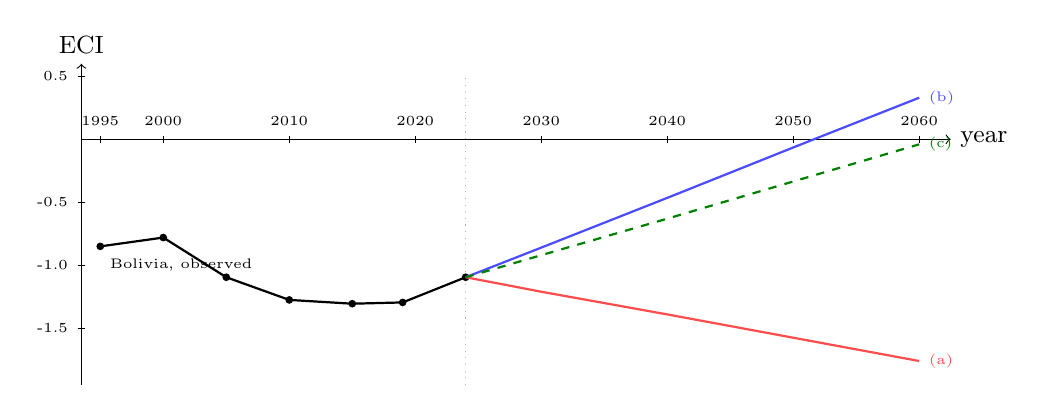
\begin{tikzpicture}[scale=0.8]
%% x = (year - 2020)/5, y = 2 ECI; coordinates printed by code/solutions/sol23.py
\draw[->] (-5.3,0) -- (8.5,0) node[right, font=\small] {year};
\draw[->] (-5.3,-3.9) -- (-5.3,1.2) node[above, font=\small] {ECI};
\foreach \x/\l in {-5/1995, -4/2000, -2/2010, 0/2020, 2/2030, 4/2040, 6/2050, 8/2060} {\draw (\x,-0.06) -- (\x,0.06); \node[above, font=\tiny] at (\x,0.06) {\l};}
\foreach \y/\l in {-3/-1.5, -2/-1.0, -1/-0.5, 1/0.5} {\draw (-5.36,\y) -- (-5.24,\y); \node[left, font=\tiny] at (-5.36,\y) {\l};}
\draw[gray!60, dotted] (0.8,-3.9) -- (0.8,1.0);
\draw[black, thick, mark=*, mark size=1.2pt] plot coordinates {(-5.00,-1.70) (-4.00,-1.56) (-3.00,-2.19) (-2.00,-2.55) (-1.00,-2.61) (-0.20,-2.59) (0.80,-2.19)};
\draw[red!70, thick] plot coordinates {(0.80,-2.19) (2.00,-2.42) (4.00,-2.78) (6.00,-3.15) (8.00,-3.52)};
\draw[blue!70, thick] plot coordinates {(0.80,-2.19) (2.00,-1.72) (4.00,-0.93) (6.00,-0.13) (8.00,0.66)};
\draw[green!50!black, thick, dashed] plot coordinates {(0.80,-2.19) (2.00,-1.84) (4.00,-1.26) (6.00,-0.67) (8.00,-0.08)};
\node[font=\tiny, red!70, right] at (8.00,-3.52) {(a)};
\node[font=\tiny, blue!70, right] at (8.00,0.66) {(b)};
\node[font=\tiny, green!50!black, right] at (8.00,-0.08) {(c)};
\node[font=\tiny, below right] at (-5.0,-1.75) {Bolivia, observed};
\end{tikzpicture}
\end{center}

\solpart{Answers} Under (a) ECI never reaches 0: it keeps falling, to $-1.761$ by 2060. Under (b) it crosses 0 in 2051.7. Under (c) it crosses 0 only in 2061.4, just after the projection horizon ($-0.041$ in 2060). Bolivia would need to sustain Korea's 1995--2019 pace for 37 years to reach the cross-country mean.

\solpart{What a trend in ECI means} ECI is a $z$-score: in each release and year it is standardized to mean zero and unit variance across the countries in the sample. Four consequences follow.
\begin{enumerate}
\item A ``trend'' is a change in \emph{relative} position. Bolivia's rise after 2019 can come from others' baskets becoming simpler, as much as from Bolivia's becoming more complex. In this case it partly reflects fuels leaving the export basket (Example~\ref{ch23:ex:epochs}).
\item ``ECI $= 0$'' means reaching the cross-country mean of that year's sample, not a fixed level of capability.
\item A $z$-score cannot trend linearly for ever: the cross-country distribution is renormalized every year, so ranks are a cleaner object. Bolivia's rank was 131 in 2019 and 123 in 2024.
\item Values are revised with each release, so a projection must state the release used. Here it is the release documented in \path{data/README.md}, \S7.
\end{enumerate}
\emph{Common mistake:} treating $\Delta$ECI like a growth rate of an absolute quantity and extrapolating it.

\end{document}
